% siminos/blog/norms.tex
% $Author$ $Date$

\chapter{Norms, distances}
\label{c-norms}
% Predrag 2012-05-04

\begin{description}

\item[2012-11-12 Predrag]
moved to here from \texttt{pipes/blog/norms.tex}.

\end{description}

\section{Norms blog}

\bigskip\bigskip
\noindent
{\color{red} The latest blog entry at the end of this chapter}
\bigskip\bigskip

\begin{description}


\label{sec:proxeq}

\item[2008-11-04 Ruslan] Excised \reffig{f:ks_prox_eq} from the rpo.tex paper,
Sect.~{\em Proximity of chaotic attractor to \eqva\ and \reqva}:

%%%%%%%%%%%%%%%%%%%%%%%%%%%%%%%%%%%%%%%%%%%%%%%%%%%%%%%%%%%%%%
\begin{figure}[t]
\begin{center}
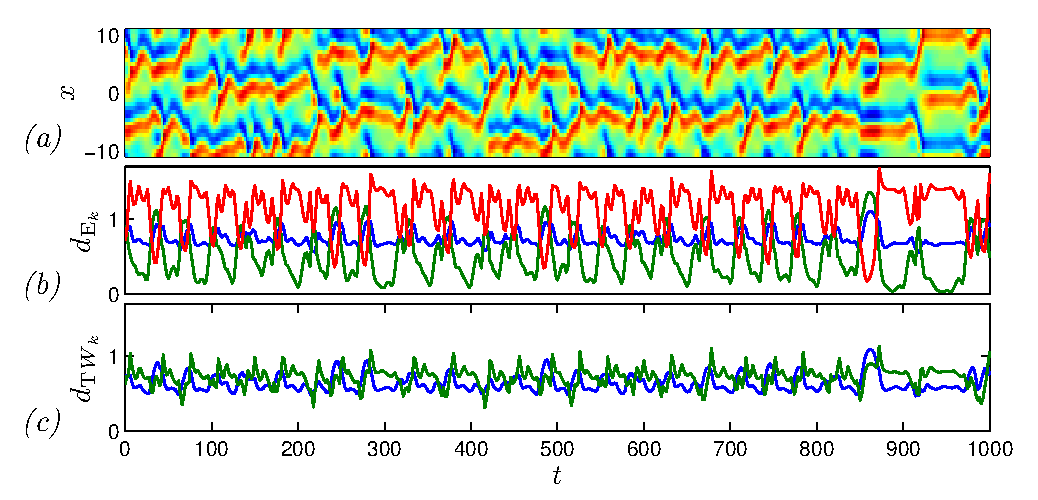
\includegraphics[width=0.9\textwidth, clip=true]{ks_prox_eq_tw}
\end{center}
\caption{  %\color{blue}
Proximity of a typical chaotic orbit of the \KSe with $L =
22$ to \eqva\ and \reqva. (a) chaotic orbit (same as in
refFig~{f:ks\_L22}); ~(b) distances of the chaotic orbit to
\eqva\ $\EQV{1}$, $\EQV{2}$, and $\EQV{3}$, are shown by
blue, green, and red lines, respectively. The distances are
measured according to \refeq{eq:proxeq}; ~(c) distances of
the chaotic orbit to \reqva\ TW$_{\pm 1}$ and TW$_{\pm 2}$,
are shown by blue, and green lines, respectively. The
distances are measured according to \refeq{eq:proxtw}.
     } \label{f:ks_prox_eq}
\end{figure}
%%%%%%%%%%%%%%%%%%%%%%%%%%%%%%%%%%%%%%%%%%%%%%%%%%%%%%%%%%%%%%%%%%

In order to illustrate the relative influence of \eqva\ and \reqva\ on
the dynamics within the KS chaotic attractor for $L = 22$, we calculated
the distance of a typical orbit, to different \eqva\ and \reqva.

The distance of a state-space point $a$ to \eqv\ $a_{\EQV{k}}$ is
measured as a Euclidean distance in Fourier space minimized with respect
to the translation of the \eqv\ by $\Shift_{\shift/L}$:
\beq
  d_{\EQV{k}} = \min_\shift \|a - \Shift_{\shift/L} a_{\EQV{k}} \|\,,\quad k = 1,2,3.
\label{eq:proxeq}
\eeq
Similarly, the distance to \reqv\ $a_{\REQV{\pm}{k}}$ is defined as follows
\beq
  d_{\REQV{k}{}} = \min_{\shift} \|a - \Shift_{\shift/L} a_{\REQV{\pm}{k}} \|\,,\quad k = 1,2,
\label{eq:proxtw}
\eeq
where we consider the distance to both $a_{\REQV{-}{k}}$ and $a_{\REQV{+}{k}}$, thus
minimizing both with respect to translation $\Shift_{\shift/L}$ and reflection $\Refl$.

The plot of $d_{\EQV{k}}$ in \reffig{f:ks_prox_eq}(b) show that \EQV{2}
has a dominant influence on the dynamics, \EQV{3} is influencing the
dynamics more intermittently, while \EQV{1} has little effect on the
dynamics.  Similarly, as shown in \reffig{f:ks_prox_eq}(c), the chaotic
orbit does not visit the neighborhoods of \reqva , so their influence on
the chaotic dynamics is also minimal.

\item[2011-11-16 Predrag] My problem is with the norm, or notion of
distance used in siminos/ksReduced. In fluid dynamics the community has
settled on
\beq
  \Norm{\ssp-\ssp'}^2  = \braket{\ssp-\ssp'}{\ssp-\ssp'} =
\frac{1}{V}
\int_\Omega \! d {\bf x} \;
(\vec{u}-\vec{u}') \cdot (\vec{u}-\vec{u}')
\,.
\label{innerproduct} \eeq
There is no compelling reason to use this {`energy norm'}, other than
that velocity fields is what is given in a numerical computation. What
norm one actually uses depends very much on the application. In the study
of `optimal perturbations' that move a laminar solution to a turbulent
one, both energy\rf{TeHaHe10} and dissipation\rf{LoCaCoPeGo11}
norms have been used.

If field $u(x,t)$ in \KSe\  is interpreted as
`flame-front velocity', the time-dependent $L^2$ norm
of $u$,
\beq
  \expctE= \Lint{\pSpace} V(x,t)= \Lint{\pSpace} \frac{u^2}{2}
  \,,
  \label{ksEnergyFreeze}
\eeq
has a physical interpretation\rf{ksgreene88} as the average `energy'
density of the flame front, in analogy to the mean kinetic energy
density for the Navier-Stokes.
I think for \KS\ it would be the safest to use
\beq
  \Norm{\ssp-\ssp'}^2  = \braket{\ssp-\ssp'}{\ssp-\ssp'} =
\Lint{\pSpace} ({u}-{u}')^2
\,.
\label{KSnormFr} \eeq
The virtue of energy norm is that it is representation independent. If
one goes to siminos/ksReduced/ invariant basis, the $2N-1$
$\SOn{2}$-invariant and functionally independent variables are
\bseq\label{eq:SO2cheb}
  \begin{align}
    \overline{b}_k &=
		    b_k\, \chebT_k\left(b_1/r_1\right)+
		    c_k\,\frac{c_1}{r_1} \chebU_{k-1}\left(b_1/r_1\right)\,, \label{eq:SO2cheb1}\\
    \overline{c}_k &=
		    b_k\, \frac{c_1}{r_1} \chebU_{k-1}\left(b_1/r_1\right)+
		    c_k\,\chebT_k\left(b_1/r_1\right)\,,  \label{eq:SO2cheb2}
  \end{align}
\eseq
for $k=1,\ldots N$, where $r_k\equiv\sqrt{b_i^2+c_i^2}$ and
$\chebT_k,\,\chebU_k$ are Chebyshev polynomials of the first and second
type, respectively. The Chebyshev polynomials $\chebT_k,\,\chebU_k$ are
degree $k$, so they tend to significantly distort the state space layout
of the attractor.

Evangelos, please confirm that you are using distance function
\refeq{KSnormFr}, not the norm
\beq
\Norm{u}  =   {\textstyle\frac{1}{2}} \sum_{k=0}^{\infty}
   (\overline{b}_k^2+\overline{c}_k^2)
\,,
\label{normNotGood} \eeq

\item[2011-12-1 Evangelos] I do not understand norm \refeq{KSnormFr}.
Take for instance a pure sin equilibrium solution of KSe and compare it
to itself under \refeq{KSnormFr} - you get zero. Now translate it by
$l<L$, and compare to the original: you get non-zero distance. Thus this
norm is not translation invariant.

I use $2\,\Norm{u}$ of \refeq{normNotGood}, since I see reduced KS as a
dynamical system defined in terms of invariant variables
$\overline{b}_k,\,\overline{c}_k$.

Please observe that although the Chebyshev polynomials
$\chebT_k,\,\chebU_k$ are degree $k$, they are functions of $b_1/r_1$ in
\refeq{eq:SO2cheb}. Therefore $\overline{b}_k, \overline{c}_k $ are not
really invariant polynomials in $b_k,\,c_k$. In fact, \refeq{eq:SO2cheb}
is equivalent to reducing to a slice with $c_1=0$. Therefore, even though
transformations \refeq{eq:SO2cheb} are nonlinear, they preserve
$r_k\equiv\sqrt{b_i^2+c_i^2}$. To see this, recall that they can be
written in the polar form
\bseq\label{eq:SO2polar0}
  \begin{align}
    \overline{b}_k &=
		    r_k\, \cos(\phi_k-k\,\phi_1)\,, \label{eq:SO2polar1}\\
    \overline{c}_k &=
		    r_k\, \sin(\phi_k-k\,\phi_1)\,.\label{eq:SO2polar2}
  \end{align}
\eseq
So any deformation of state space is a result of symmetry reduction
(identification of points along group orbits) and the discontinuity at
$r_1=0$.

If we were to follow Tuckerman's recipe and multiply \refeq{eq:SO2polar}
by $r_1^k$ we would indeed have invariant polynomials of order $k+1$ in
the $b_i,\,c_i$. In siminos/ksReduced, we try to keep state-space
distortion to a minimum, therefore multiplying by $r_1$ (or $r_1^2$).

\item[2012-02-23 PC]
\index{recurrence!plot}
In literature on \emph{recurrence plots} I see Euclidean, Manhattan, and
maximum norms. The maximum norm for defining distances in \statesp\ is
reputed to have lower computational demands than other norms.

\item[2012-05-04 Predrag] Asked Francesco's colleague
\HREF{http://www.ece.gatech.edu/research/labs/lccv/}{Tony Yezzi} about
norms for turbulent Lagrangian flows. He had an original idea on how to
measure distance between two Lagrangian twirls of spaghetti: Think of
particle tracers embedded in a turbulent flow as 4\dmn, 3 spatial
dimensions, a time dimension along the spaghetti. 3 bounded dimensions
are nice, as you can think of them as three color channels, and express
the spatial position at time $t$ by a dot whose color is given by the
3\dmn position. Then the Lagrangian state of the fluid at time $t$ is a
3\dmn\ color picture, and the distance between two nearby fluid states is
given by the $L2$ distance between color pictures.

\item[2012-05-29 Predrag] Kreilos and Eckhardt\rf{KreEck12}
use `the cross-flow energy', i.e.\ the amount of energy in the
  flow components transverse to the laminar base flow,
  \beq
  E_{cf} = \frac 1V \int_V\left(v^2 + w^2\right)\mathrm dV,
  \ee{KreEck12norm}
{\bf [Ashley]}: It is difficult to make a strong case either for
or against the cross-energy norm.  Kerswell and Tutty\rf{KeTu06} essentially
did the same for correlations (their $I_{uv}$) that has frequently been
adopted, despite that they say it should be used with caution, i.e. check
other variables too to ensure a real correlation, namely, dissipation $D$.
In practice it looks like the $u\!-\!v$ measures can look similar for states
that are out in $D$ by a factor of 2-5.  To be honest, maybe $D$ would have
been better, but I suspect $E_{cf}$ was chosen purely because figure 3 looks
nice.



                                        \phantomsection\label{newNorm}
\item[2012-07-25 Predrag]
So far we are measuring the distance $\Norm{\ssp}^2=\braket{\ssp}{\ssp}$ in
terms of the Euclidean inner product, or $L^2$ norm
\beq
\braket{\ssp}{\slicep} = \sum_i^d {\ssp}_i \slicep_i
    \,,\; \qquad
x, y \in \pS \subset \reals^d
	\,.
\ee{innerR}
Any representation of a compact group $\Group$ is fully
reducible\rf{Hall03}. The invariant tensors constructed by contractions
of $\Lg_a$ are useful in identifying irreducible representations. The
simplest such invariant is
\beq
{\Lg}^{\dagger} \cdot \Lg = \sum_m C_2^{(m)} \, \id^{(m)}
\,,
\ee{QuadCasimir}
where $C_2^{(m)}$ is the quadratic Casimir for irreducible representation
labeled $m$, and $\id^{(m)}$ is the identity on the irreducible subspace
$m$, 0 elsewhere. For compact groups $C_2^{(m)}$ are strictly
nonnegative. $C_2^{(m)} =0$ if $m$ is an invariant subspace. For \SOn{2}
it is simply $C_2^{(k)} =k^2$, $\id^{(m)}$ is $[2\!\times\! 2]$ unit matrix,
where $k$ refers to the $k$th Fourier
mode.

The dot product of two tangent fields % in \refeq{min4}
is a sum of inner
products weighted by Casimirs \refeq{QuadCasimir}, % as in \refeq{min5}
\beq
\braket{\groupTan(\ssp)}{\groupTan(\slicep)}
   = \sum_m C_2^{(m)} {\ssp}_i\, \delta_{ij}^{(m)} \slicep_j
\,.
\ee{braket}
The slice condition thus preferentially weighs higher Fourier modes. If
we think of the norm as Sobolev norm (probably best to ignore this
remark) it would be natural to have it as unit norm on the product of
tangents, which  means we should change \refeq{innerR} to
\beq
\braket{\ssp}{\slicep}
   = \sum_{m \neq 0} {\ssp}_i\, \frac{\delta_{ij}^{(m)}}{C_2^{(m)} } \slicep_j
\,.
\ee{braketCas}
This would suppress higher Fourier modes, on hopefully tame the fast
rotations observed by Ashley and Sebastian in pipe, respectively
baroclinic  flows.

$\Lg$ is what it is, I do not think we have a freedom
to change it, as $\groupTan(\ssp)$ is no more a group
tangent, so I cannot think of an argument that would allow for
modification of \reffig{fig:thetadot}\,(a).
It would be legal to try for $\SOn{2}$
($\Un{1}$)
\beq
\braket{\ssp}{\slicep}
   = {\ssp}_i\, \delta_{ij}^{(0)} \slicep_j
      +
   \sum_{m \neq 0} {\ssp}_i\, \frac{\delta_{ij}^{(m)}}{|m|^\alpha} \slicep_j
\,,\qquad \alpha > 1, \alpha \in \reals
\,.
\ee{braketAsh}
The norm could be inverse of any monotonely increasing function of $|m|$,
though I would prefer it to be as fast as $|m|^2$ or faster. For the $|m|^2$
case we might be able to develop a Green's function (or energy?) argument why to
use it - for an arbitrary function I see no way to justify it...

It does not collide with the compensatory norm \refeq{compensNorm1},
as that rescales the overall prefactor for each \SOn{2} separately.



{\color{red} Please try it!} a very simple change in the slicing condition that
should reduce the number of charts along short recurrent orbits.

\item[2012-07-26 Ash]
A minor point -- what about the division by zero for the $m=0$ term in
\refeq{braketCas}? (For the inner product with a tangent this doesn't
matter, as the tangent has no $m=0$ term.)

\item[2012-07-26 Predrag] I think it's best to fix the $m=0$ term in
the norm to be $1$ by hand, meaning that in the invariant subspace the distance
is Euclidian, and mess with high $|m|$ in order to suppress high frequencies.

$m=0$ term is the average of the function, so if that is 0, we are OK.

In Sebastian's \texttt{siminos/baroclinic/} simulations it is clear that
on stays on a given chart for very short time because there is lots of small
scale vortices moving fast. The physics of suppressing high frequencies would
be that we care about large scale structures, and the small scale vortices would
act as a noisy superposition on the slow large-scale motions.





                                        \phantomsection\label{negSobol}

\item[2012-07-26 Predrag] I think we can probably make a good argument
that the group manifold should be a
\HREF{http://en.wikipedia.org/wiki/Sobolev_space\#Sobolev_spaces_with_integer_k}
{Sobolev space} $W^{1,\infty}$ with respect to group parameter
derivatives - the group orbit is a smooth manifold. I have argued some
time ago for Ruslan Davidchack somewhat inchoately that for \KS\ Fourier
expansion of $u(x)$ ({\bf [2012-03-25 Predrag to Evangelos]}) that the
important, nonlinearly coupled Fourier modes contribute significantly
for any magnitude not smaller than $1/m$ for the $m$th mode.'' If they do
this for $k \to \infty$, the partial derivative $u_x$ is not defined, and
that would be a disaster. Which probably means for Navier-Stokes that we
can demand that solutions belong to $W^{2,\infty}$ which would make it
legit to use even stronger suppression of high Fourier modes, with norm
diagonal $\propto (C_2^{(m)})^{-2}$.

Guys, please think this through, bring your erudition to justify our new
fancied-up norms. True confessions - I have never had any course about
differential equations higher than undergraduate linear differential
equations, replete with boring Laplace transforms.

\item[2012-07-31 Predrag] Sara says `new norm' is an example of a `filter' in
engineering; they smooth Brownian noise, turn it into time-correlated colored
noise. In particular, $\omega^{-1}$ and $\omega^{-2}$ filters
are common, we should find what engineers call them.

I would distinguish between band-pass filters (which throw away parts of
the spectrum, and re thus what we call spectral truncations) and filters
like the `new norm' which weigh modes differently, but lose no modes - if
something is computed in the `new norm' it can always be inverted and the
corresponding full state reconstructed.

\item[2012-07-29 Predrag] With the `new norm' working better for slicing, we
should re-examine everything that depends on the choice of a norm:
\begin{itemize}
  \item Our Poincar\'e sections depend on the choice of a norm, just like
  the slices do. If we switch to the `new norm', the invariant manifolds
  are smoother, neighborhoods larger, and fewer sections might do the
  job.
  \item Our Newton routines use Euclidean norm (that is clear if you
  derive Newton from minimizing the quadratic error function, as in
  \refref{CvitLanCrete02}). If we switch to the `new norm', the
  invariant manifolds are smoother, neighborhoods larger and searches
  might be easier and converge faster.
  \item $1/m^2$ is the Fourier transform of the Laplacian operator
  $\partial^2$. So for pipe and plane flows we should also use the `new
  norm' in the wall-normal directions. For channel flows that means using
  the wall-normal Laplacian in Chebyshev basis, for pipe flows using
  radial Bessel functions basis.
\end{itemize}

\item[2012-08-01 Predrag] The `new norm' is not nameless any more.
It is the negative Sobolev norm $H^{-1}$ (more generally $H^{-\alpha}$)
\beq
\Norm{\ssp}^2
   =
   \sum_{m \neq 0} \frac{\ssp_m^2}{|m|^2}
\,.
\ee{Sobolev-1}
Image-reconstruction people deploy tempered
distributions belonging to the negative Hilbert-Sobolev spaces
$H^{-s}, \;\; ( s > 0 )$ for textured
components. Budi\v{s}i\'c and Mezi\'c\rf{BudMez12} are big fans too:


Trajectories are aggregated into coherent structures by a criterion of
similarity embodied in a distance function between trajectories. The
choice of the distance function determines the type of coherent
structures we obtain. In this work, we chose to work with the empirical
distance, which compares two trajectories based on residence times.
%\cite{Mathew:2011ev}.
Instead of working with the empirical distance
directly on the state space, we use a distance on the ergodic quotient
that is equivalent to it, thus converting the analysis of dynamics into
analysis of geometry of the ergodic quotient. [...]

[...] the metric induced by the norm on a negative-order
Sobolev space of measures can be used [...]. The distance
\begin{align}
  \begin{aligned}
    \mathcal{D}_{-s}(\mu_x,\mu_y) &\triangleq \norm{\tilde F(x) - \tilde F(y)}_{2,-s}\\
    \norm{\tilde F(x) - \tilde F(y)}_{2,-s}^2 &= \sum_{k \in \mathbb{Z}^D}
    \frac{ \left\lvert{\tilde f_k(x) - \tilde f_k(y)}\right\rvert^2 }{ \left[ 1 +
        \left(2\pi \norm{k}_2 \right)^2\right]^s },
  \end{aligned}\label{eq:negsobdist}
\end{align}
is easily computed as a weighted sum of Fourier coefficients,
\[
\tilde
F(x) \triangleq \left( \dots, \tilde f_k(x), \dots \right)_{k \in \mathbb{Z}^D}
\]
of measures involved. The order $s$ of the Sobolev space is selected
based on the dimension $D$ of the domain of measures $\mathcal M$  as $s
= (D+1)/2$. Using $\mathcal D_{-s}$ instead of $\mathcal D$ does not
change the resulting topology, as the empirical metric and the $H^{-s}$
with the order $s = (D+1)/2$ are equivalent.
''
It seems (to Predrag) that the numerator in \refeq{eq:negsobdist} has
a `1~+' term just to fudge over the $k=0$ term... Also $s = (D+1)/2$ seems
pulled out of the hat.

Charlie Doering says they (with
\HREF{http://www.math.wisc.edu/~jeanluc/preprints.html} {Jean-Luc
Thiffeault}) use it in their papers with  as a measure of mixing of
particles in passively advected flows. The problem there is that $L^2$
and all $L^p$ norms are conserved, as can be see by multiplying
\[
\frac{\partial~~}{\partial t} \theta
  + u \cdot \nabla \theta =0
\]
by $\theta$ (or $\theta^{p-1}$) and integrating. For coarse nonuniform
distribution $H^{-\alpha}$ is dominated by long wavelengths, and its
vanishing is a measure of mixing.

While  $L^2$ is singled out by Perseval's theorem (its Fourier transform
is also $L^2$), Charlie sees nothing special about the  $H^{-1}$ norm.

\item[2012-08-02 Predrag]
\HREF{http://www.math.wisc.edu/~jeanluc/preprints.html} {Jean-Luc
Thiffeault} reviews Sobolev norms in Sect.~3 of \arXiv{1105.1101} - he also
defines norm \refeq{eq:negsobdist}, but prefers to use our 'new norm'
(now called `the seminorm on the homogeneous space') which has a more
intimate connection with solutions of the advection-diffusion
equation.'' If average of the function is zero, 'new norm' is a true norm.
In passive mixing, the time evolution of the $H^{-1}$ norm of advected scalar
has explicit inverse Laplacians in it, his eq.~(3.14). Mixing people also work
with the $H^{-1/2}$ norm of a concentration field.

\item[2012-08-03 Igor]
\emph{Applied Koopmanism} by
Marko Budi\v{s}i\'c, Ryan M. Mohr and Igor Mezi\'c, \arXiv{1206.3164}
is our latest that attempts to review what we have done
with Koopmania in the past and reviews and gives references for negative
Sobolev.

\item[2012-08-15 Humbledt] (Beijing early morning)
'Negative Sobolev norm' does not roll off the tongue easily. Maybe define it once
in the article (the one that we are still responding to referees to, or the famed
Phys. Rev. Letter?), then
just say '$H^{-1}$-norm' from then on?

\item[2012-09-18 Humbledt] Paul Goldbart has never used $H^{-1}$-norm but
he hears a tiny bell tinkle: inverse Laplacian norm is perhaps used in
Kleinart's field theory book, in current-current correlations?

\item[2012-11-10 Humbledt] Jean Bellissard has much to say about Sobolev
norms, starting with Serge� L'vovich work on atom bomb
(Sobolev and Kantorovich were
involved in the Kurchatov's 1943 project Enormous''), and all the way
to the Singer-Atyah index theorems. (A side note: Google blows out Bing in
"Sobolev  Singer-Atiyah index theorem" search.)

\noindent
A few notes from (a bit odd, and not informative) \arXiv{0801.4174}:

Leonid Kantorovich created the theory of distributions (1935), which was
then taken on by Laurent Schwartz. Sobolev also published his ideas in
1935. While working on the bomb, Sobolev wrote {\em Some Applications of
Functional Analysis in Mathematical Physics}. The work on the bomb taught
him the importance of finding a reasonable solution rather than proving
the existence of a solution to an abstract problem. The generalized
derivatives in the Sobolev sense do not obey the Eulerian definition of
function. Differentiation by Sobolev implies the new conception of
interrelation between mathematical quantities. A generalized function is
determined implicitly from the integral characteristics of its action on
each representative of some class of test functions that was chosen in
advance.

From Antony Wassermann
\HREF{https://www.dpmms.cam.ac.uk/~ajw/AS10.pdf}{notes}:
The Sobolev spaces $H^{k}(V )$
are the Hilbert space completions of $\complex^{\infty}(V )$ for the norms
\(
\norm{\xi(k)} = \braket{(I + D^2_V )^k\xi}{\xi}^{1/2}
\,,
\) doe $k \in \reals$, usually half-integer.
Reading this is really rough going for me, but key ingredients seem to be
solving the eigenvalue/eigenfunction problem associated with a given Laplacian
(here only the trigonometric polynomials case is discussed),
and the Sobolev's embedding theorem.

\item[2013-03-06 Humbledt] Heard a talk by
\HREF{http://www.rosslhatton.com/} {Ross Hatton},
reading Ross L. Hatton and Howie Choset {\em Kinematic Cartography for Locomotion
at Low Reynolds Numbers}:
In motion planning and locomotion analysis, it is often
useful to consider the ``distance'' between two configurations
or the ``length'' of a given trajectory through the configuration
space. These quantities are often defined by a simple Euclidean
metric on the system parameters, but several limitations make
this approach unsatisfactory for many applications. First, it inherently
requires the determination of scaling factors to relate
heterogeneous configuration parameters, such as translation
and rotation. Second, it includes an often-false underlying
assumption that the costs for changing configuration are both
uniform and orthogonal -- i.e., that they depend neither on the
current configuration nor on any coordination between changes
in different parameters. [...]

These problems bear a strong resemblance to map projection
issues considered in theoretical cartography. Drawing on
established practices from the cartographic community [1],
[2], we have developed a means for representing how given
parameterizations distort effort metrics on the configuration
space and then reparameterizing the shape spaces to optimally
flatten these metrics. Such reparameterization ensures that the
shape space is faithfully represented for plotting or sampling
purposes, in much the same way that certain maps are more
accurate than others at representing the surface of the globe.

[1] M. Tissot, Memoire sur la Representation des Surfaces et les
Projections des Cartes Geographiques. Paris, France: Gautier-Villars,
1881.
\\
~[2]~A. Niermann, ``A comparison of various advantageous cartographical
representations,'' Master's thesis, Universit\"at Stuttgart, Stuttgart,
Germany, June 1983.

We first introduce a power-based configuration distance metric that
directly corresponds to the energy dissipated while changing shape.
Working with this metric allows for true comparison of configuration
distances and trajectory lengths, abstracting away the need to consider
pacing along trajectories. [...] By applying the dissipation metric and
cartographic reparameterization, we directly compare the locomotive
efficiencies of articulated and continuous swimmers both in general and
for specific optimized strokes.


Read also: ``Measuring shape with topology'' by
Robert MacPherson and Benjamin Schweinhart\rf{MacSch12}
(click
\HREF{http://ChaosBook.org/library/MacSch12.pdf} {here}).


''


\end{description}
